%% ==============================
\chapter{Concept}
\label{sec:concept}
%% ==============================
Questions to ask:
\begin{enumerate}
    \item What is the high level concept of your work?
    \item What are important design decisions?
    \item Why did you choose this concept and what are the alternatives?
    \item What are drawbacks of your concept?
    \item How does your concept exceed existing approaches?
    \item How does this concept solve your research question?
\end{enumerate}

\begin{enumerate}
    \item Creation of semantic hierarchical graphs
    \item Algorithms with Pseudocode
    \item Usage of semantic informations
    \item Speed zones, no-go zones special locations
    \item 
    \item General concept H-Graph solver and straight path planner working togehter with ROS2
    \item concept hierarchy creation and map preprocessing
    \item concept straight path planner
    \item concept H-Graph building and planning problem: optimality solved with try all possible
    \item concept integration in Nav2 stack
    \item concept process with behavior tree
\end{enumerate}

The problem of multi-floor navigation can generally be split up in the following six sub-problems:

\begin{enumerate}
    \item \textbf{Model the environment}\\
    Output: Gridmaps, locations of hierarchical connections
    \item \textbf{Hierarchy creation}\\
    Output: Room segmentation, H-Graph
    \item \textbf{Generate roadmaps}\\
    Output: Precalculated paths between hierarchies
    \item \textbf{Hierarchical planning}\\
    Output: Collision free path from start to goal
    \item \textbf{Execute with a mobile robot}\\
    Output: Behavior tree for multi-floor navigation
    \item \textbf{Interact with infrastructure}\\
    Output: Hardware interfaces, Behavior trees
\end{enumerate}

This chapter outlines the concepts of this work for solving these problems. Also the limitations of the scope of this work are highlighted. The fundamental step for navigating in a multi-floor environment is gathering information of the environment and creating a model which represents all relevant information for navigation in the specific buildings. In minimum this includes a representation of the drivable are on each floor. This can be in a form of a discretisized gridmap, a 3D Voxel representation as Octomap \cite{hornung_octomap_2013} or other visual markers. WIthin the so defined coordinate system, the locations of all hierarchical connections have to be marked. These are doors between rooms, elevators between floors or connections between buildings like bridges or ramps. For maximum autonomy the goal would be to generate those autonomously while exploring the whole environment. Although frameworks for autonomous exploration and mapping exist, this is not in the scope of this work. To model the test environment in the lab and in simulation, manual gridmaps were created with \gls{slam}. The locations of elevators and connections between buildings were created manually. Only the connections on the lowest hierarchical level, which are doors between rooms, were created automatically from the provided gridmaps as part of the room segmentation.

Hierarchy creation is done in two steps. First the model of the environment has to be split up into its respective hierarchical structure, second an H-Graph is created which represents the hierarchical connections and holds the individual parts of the environment on its lowest level. For the segmentation of rooms from gridmaps the marker-controlled watershed algorithm from \cite{parvati_image_2009} was used. Only the automatic hierarchy creation of rooms from gridmaps is scope of this work. Higher levels of hierarchies are created manually. To find the hierarchical bridge points, in this case: doors between rooms, The optimal locations are extracted during the segmentation process. This is inspired by the approach from \cite{ryu_hierarchical_2020}. Details to the specific implementation follow in Chapter \ref{sec:hierarchy_creation}.

The generation of roadmaps follow the principles presented in the problem statement. This means the goal is to find paths that are straight, deterministic and human-predictable. The concept in this work accounts for that by generating straight paths that are mostly parallel to the walls. This is done by first rotating the gridmap to be parallel with the axis of the coordinate frame and then iteratively generating the largest free rectangle in each room. Thus this straight path planner is called \gls{ilir}. These rectangles are then merged to one single polygon and connected with all doors to adjacent rooms. The advantages of this approach are the following:

\begin{enumerate}
    \item Deterministic, the robot takes the same path every time
    \item Straight paths following the walls
    \item Human-predictable for bystanders
    \item Reduce fear for passengers
    \item Avoid disturbance of public space
    \item Can be represented as a graph and searched very fast
\end{enumerate}

The drawbacks of \gls{ilir} are that this planner is not providing optimal paths and includes sharp 90 degree turns. The rectangular corners are later smoothed by the controller of the \gls{nav_2} stack which follows the generated path with a maximum turning angle. This precalculated roadmap now connects all hierarchical neighbours like other rooms by doors and other floors by elevators. These roadmaps provide the basis for path planning in each room. arbitrary start or goal connections are later connected to this graph. The graph representing the roadmap is the lowest hierarchy level in the \gls{h_graph}. Implementation details are presented in Chapter \ref{sec:roadmap_generation}.

%% ==============================
\section{Hierarchical Planning}
\label{sec:hierarchical_planning_method}
%% ==============================

Once an H-Graph of the environment is created, the next problem is solving the planning for a specific pair of start and goal locations. Each can be on different floors in completely different buildings. This requires planning over multiple subgraphs. In this concept, the single hierarchical entities like rooms, floors or buildings represent a node in the graph one hierarchy level higher. In Figure \ref{fig:hierarchical_planning} each hierarchical level of the \gls{iras} research campus can bee seen. 

\begin{figure}[h]
    \captionsetup[subfigure]{justification=centering}
    \centering
    \begin{subfigure}{\textwidth}
      \centering
      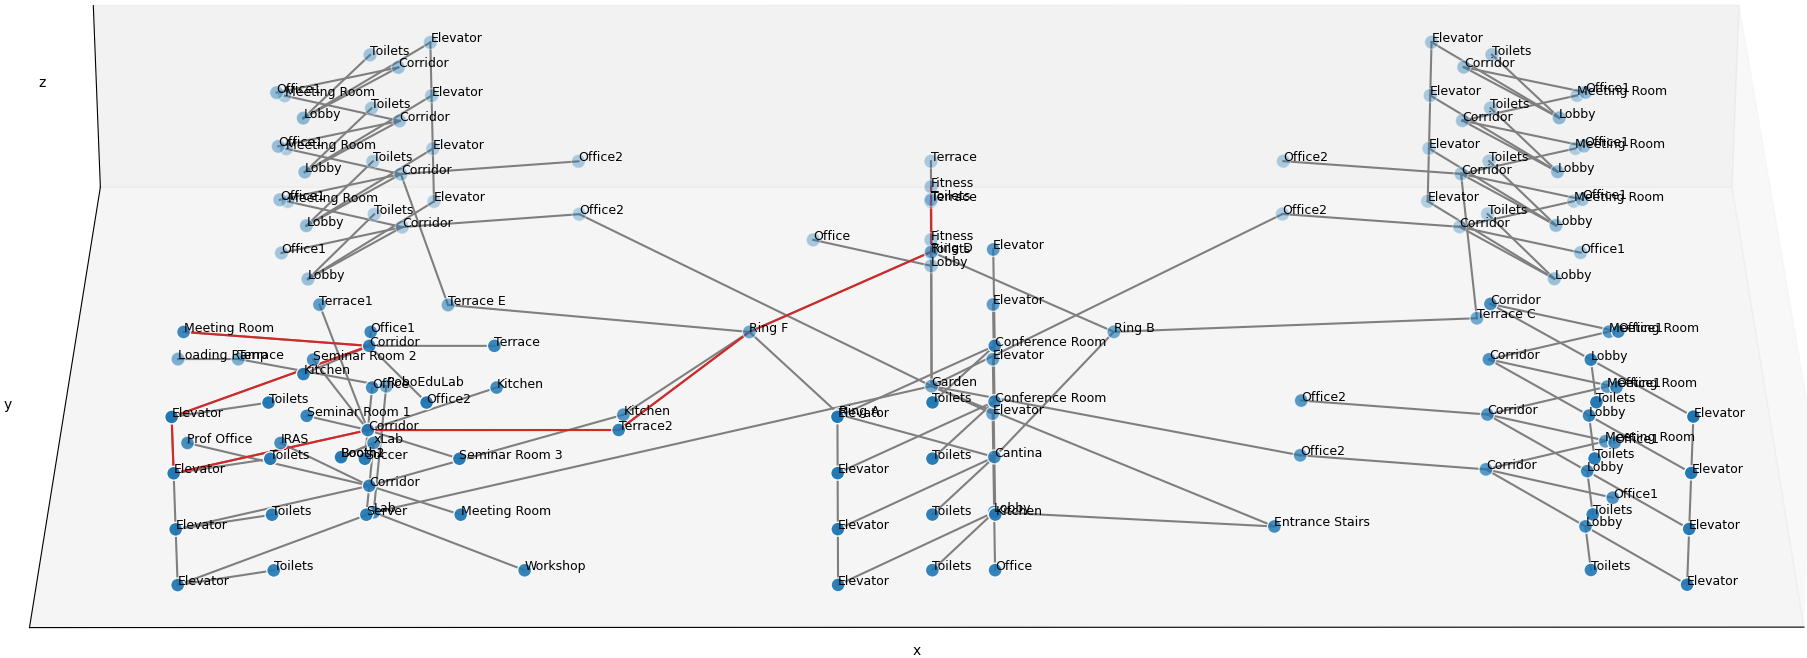
\includegraphics[width=\textwidth]{figures/40_concept/ltc_graph_complete.png}
      \caption{Overview graph just for visualization}
    \end{subfigure}
    \begin{subfigure}{.4\textwidth}
      \centering
      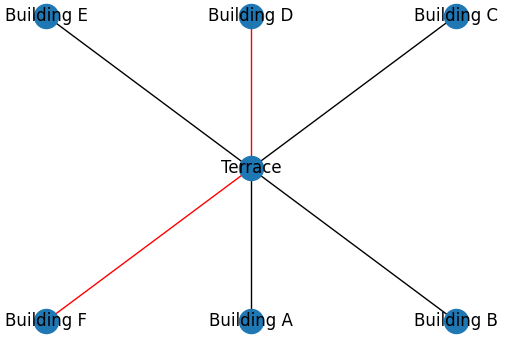
\includegraphics[width=\textwidth]{figures/40_concept/ltc_graph_campus.png}
      \caption{Graph of research campus (H4)}
    \end{subfigure}%
    \begin{subfigure}{.6\textwidth}
      \centering
      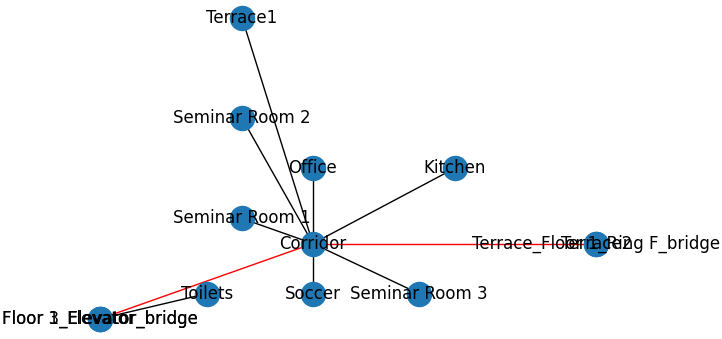
\includegraphics[width=\textwidth]{figures/40_concept/ltc_graph_floor_2.png}
      \caption{Graph of Floor 2, Building F (H2)}
    \end{subfigure}
    \begin{subfigure}{.2\textwidth}
      \centering
      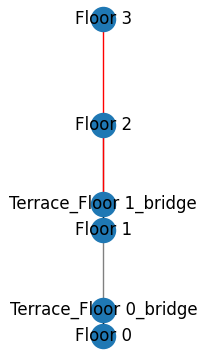
\includegraphics[width=\textwidth]{figures/40_concept/ltc_graph_building_f.png}
      \caption{Graph of Building F (H3)}
    \end{subfigure}%
    \begin{subfigure}{.8\textwidth}
      \centering
      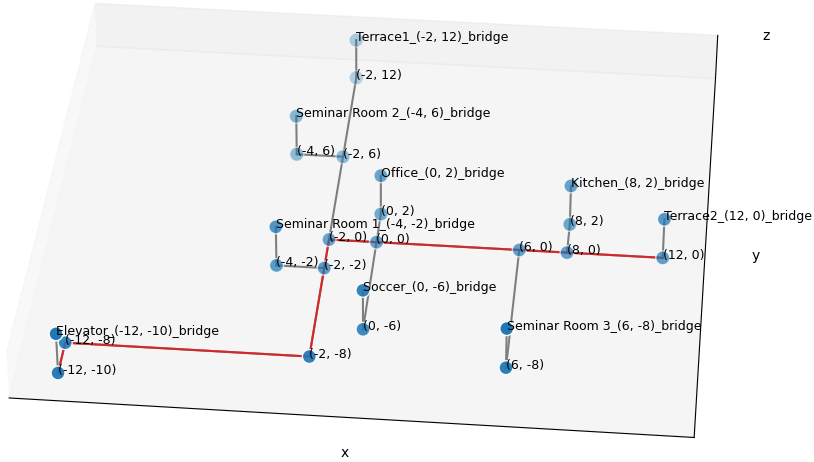
\includegraphics[width=\textwidth]{figures/40_concept/ltc_graph_corridor.png}
      \caption{Graph of Corridor on Floor F2 (H1)}
    \end{subfigure}
    \caption[Hierarchical path planning with 4 hierarchy levels]{Hierarchical planning with 4 hierarchy levels (H1 - H4) and solution path from Meeting Room to Fitness Studio (red). a) Visualization of all rooms from level H2 in a single graph only for orientation. b) Buildings of the campus. c) Rooms of the second floor d) Floors of building F. e) Roadmap of the corridor on the lowest hierarchy. Bridges to other adjacent hierarchies are in z +1 and have no path cost.}
    \label{fig:hierarchical_planning}
\end{figure}

The benefit of this approach is the more intuitive representation, the better mapping of the corresponding gridmap to the nodes and a smaller and less denser H-Graph. The drawback of this concept is a more complex hierarchical planning algorithm because in the top-down search the absolute distances of the lower levels are not known. This results in the requirement of calculating all possible solutions to the goal on one hierarchy level and then exploring each node on its corresponding subgraph and calulating all possible solutions in this graph aswell until the lowest hierachy is reached. From this top-down search multiple possible paths a reconstructed and combined on the lowest level. In the end all feasible paths have to be compared in length to choose the optimal path. In comparison, Seder \cite{seder_hierarchical_2011} uses the bridge points as hierarchy nodes in the graph. this way all possible paths can be easily precalculated and already on the highest hierachy level only the shortest path has to be explored deeper. This drawback of the current concept can be accounted for by two solutions: First by introducing a heuristic like euclidean distance which estimates the minimum distance between nodes on a lower level and thus enables it to search with a A* instead of dijsktras algorithm for the optimal path. The second solution would be to provide a mapping on the parent node which holds all the possible combinations of connections of possible start and goal nodes in the subgraph and its corresponding costs. This can be precalculated from bottom to top and then used later to efficiently search from top to bottom. Both of these solutions are currently not implemented. This concept uses the approach of exploring all possible solutions to its maximum depth and then comparing for the shortest solution.

%% ==============================
\section{Execution with a Mobile Robot}
\label{sec:execution}
%% ==============================
To bring all of the previous concepts together a Behavior Tree is used to coordinate all the different subtasks. Because the goal of this work is to enable a real robot to navigate between different floors, the problems 1. - 4. have to be wrapped in ROS 2 nodes to interact with the rest of the robots hardware and to be able to listen to the commands from the Behavior Tree framework that is used. In Chapter \ref{sec:navigation_stack} the default \gls{nav_2} stack and its architecture for mobile robot navigation was presented. This modular architecture is now expanded with custom planner plugins and integrated into the simulation and the real world PeTRA robot. In Figure \ref{fig:concept_nav2} the expanded architecture can be seen. 

\begin{figure}[h]
    \centering
    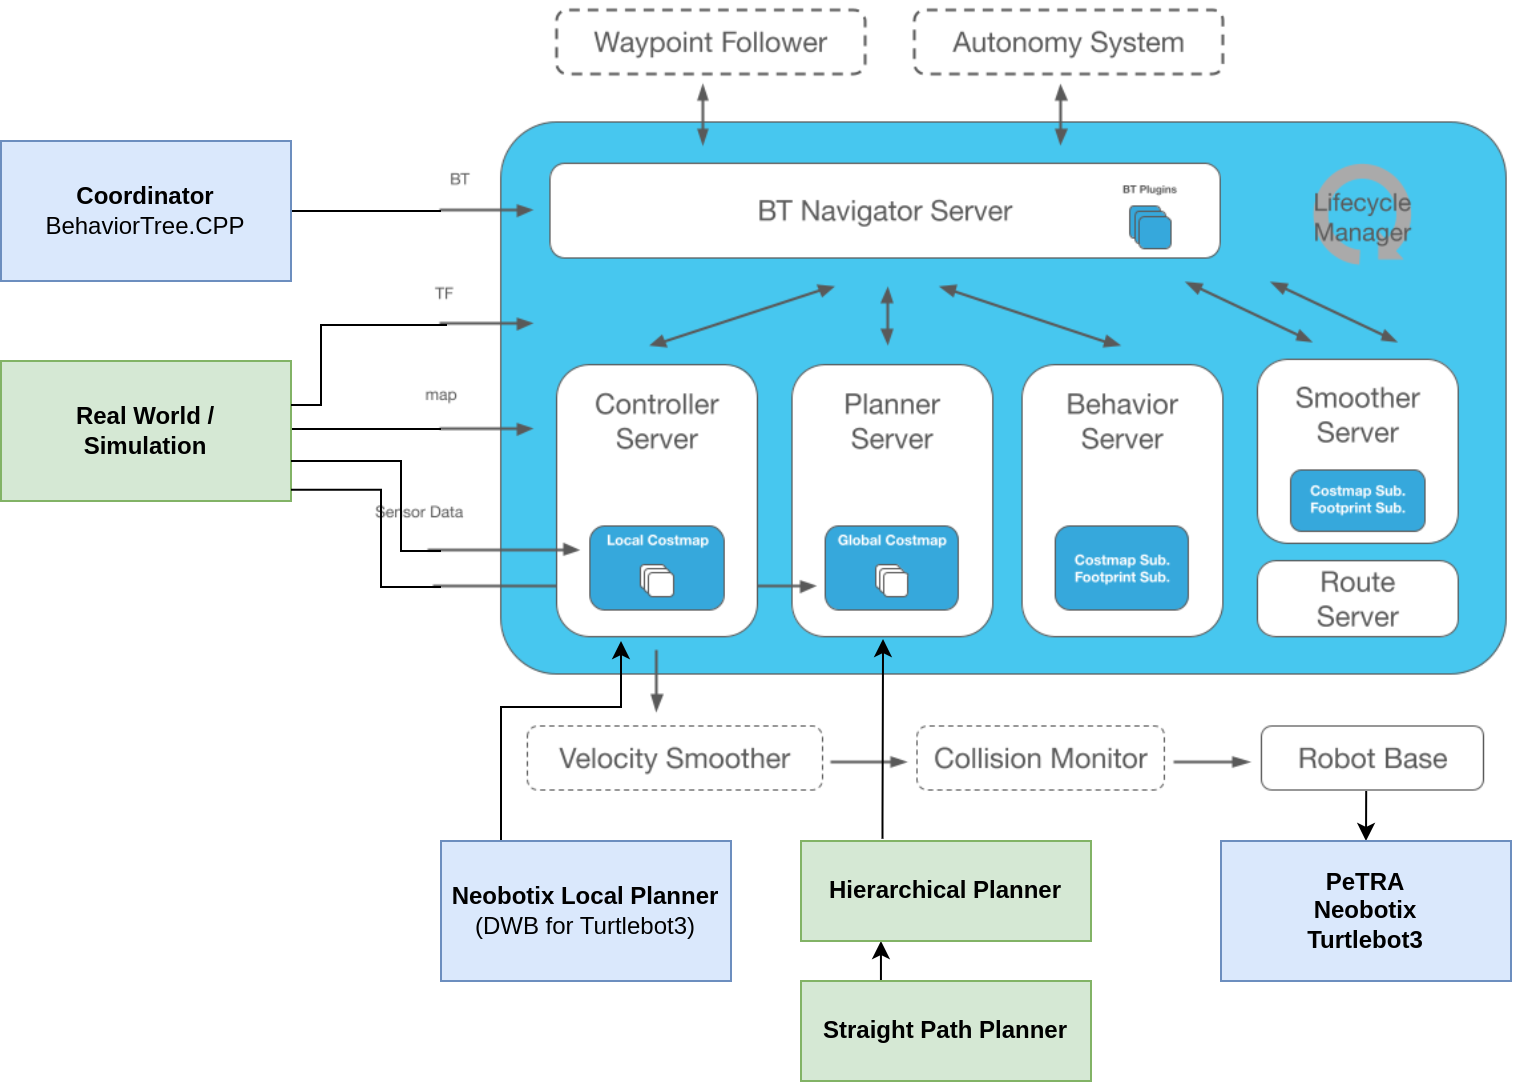
\includegraphics[width=\textwidth]{figures/40_concept/concept_nav2.png}
    \caption[The architecture of the NAV2 stack extended with custom nodes for hierarchical planning and (simulated) hardware]{The architecture of the NAV2 stack extended with custom nodes for hierarchical planning and (simulated) hardware. Blue components were taken from the community, green components were developed in this work.}
    \label{fig:concept_nav2}
\end{figure}

The modular server-client architecture for the Controller, Planner, Behavior and Smoother allows to swap the default implementations. In this case the Controller, also known as local planner, from the Neobotix MPO\_500 robot is used. This robot was used as development platform for PeTRA and its planners provided better accuracy and customizability then the default \gls{dwa} controller. For this reason the Neobotix local planner \cite{pradheep_krishna_neobotixneo_local_planner2_2021} is used for PeTRA as well as for the MPO\_500 in real world and simulation. Only for testing with the Turtlebot3 the DWB Controller was used which is an advancement of the DWA controller. As global planner the previously described Hierarchical Planner developed in this work is used. For roadmap generation this planner plugin uses the \gls{ilir} straight path planner. The inputs to this navigation system come from the robot hardware whereby it does not matter if the sensor information is retrieved from the real world or from the gazebo simulation. The high-level task coordination is done by the Coordinator node which uses the BT framework BehaviorTree.CPP \cite{auryn_robotics_behaviortreecpp_2023}. In Figure \ref{fig:concept_uml} the interactions between these components is described in more detail. The diagram is loosely based on the \gls{uml} representation of these classes.

\begin{figure}[h]
    \centering
    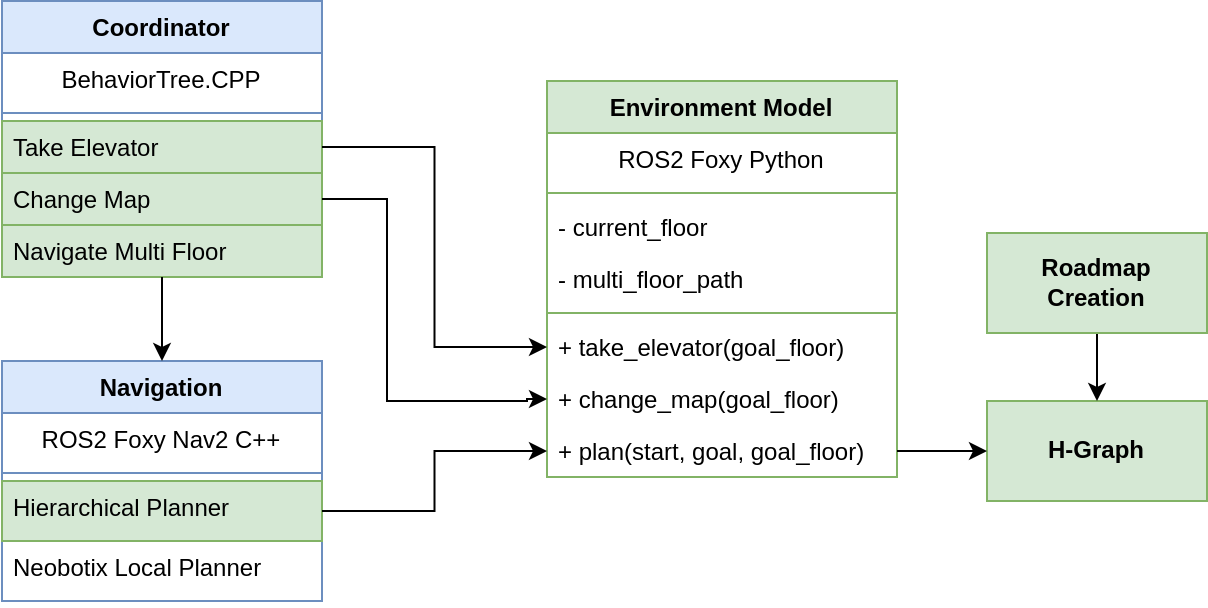
\includegraphics[width=0.75\textwidth]{figures/40_concept/concept_uml.png}
    \caption[Interactions between the custom components for multi-floor navigation]{Interactions between the custom components for multi-floor navigation. Blue components were taken from the community, green components were developed in this work.}
    \label{fig:concept_uml}
\end{figure}

The core component for storing information about the environment and thus enabling the multi-floor navigation is the Environment Model. This ROS 2 node stores the current floor, holds the H-Graph with the gridmaps for all other floors and executes floor and map changes by updating the respective information. The process for a multi-floor navigation task is as follows: First, the H-Graph of the environment is created with the precalculated roadmap from the ILIR planner and stored by the Environment Model. A single planning request is triggered by the current BT of the Coordinator through the Navigate Multi Floor action. This is processed by the standard action server of the \gls{nav_2} stack. The loaded custom planner plugin for the Hierarchical Planner sends a planning request to the H-Graph of the Environment Model. There the hierarchical planning is executed considering additional information like the current floor. This is important because the path returned by the Environment Model only contains the path on the current floor that can be executed by the \gls{nav_2} stack with the currently loaded map. All other paths on different floors and hierarchy levels are stored in the private multi\_floor\_path variable. It is necessary to store this information although only the path on the current floor is executed. This is used to know which gridmap should be loaded next and which elevator and floor number has to be called to reach the final destination. Once the robot reaches the elevator and therefor its goal on the current map, the BT triggers the Take Elevator and then the Map Change. For the latter the Environment Model loads the new gridmap updates the internal state information. Take Elevator is only served by the Environment Model to give information about the next target floor like, floor number, exact waiting pose in front of the elevator and location of the control panel inside the elevator. This is not the complete action fro Take Elevator as the BT then executes the necessary actions to perform the real operation of calling the elevator, choosing the floor, driving into the elevator and exit it on the target floor. For detailed information on the BT which coordinates these behaviors, see Chapter \ref{sec:multi_floor_behavior_trees}. In the most simple case in the hospital simulation. This action only triggers a teleport of the robot model of the simulation to the corresponding position in front of the elevator on the target floor. After the robot reaches the target floor the Coordinator again triggers an Navigate Multi Floor Action but this time receives the path on the new floor from the Environment Model.

The last problem to solve from the list at the beginning of this chapter is the interaction with the infrastructure. As mentioned before, it is the responsibility of the Coordinator to trigger all necessary actions to perform an elevator transition. But the specific implementation of this BT depends very strongly on the available infrastructure, the degree of automation and the capabilities of the robot itself. The same applies to all same-level connections like doors between rooms. These can also be very different from doors with handles, an button to open automatically to a revolving door. As this work is part of the research project PeTRA with multiple hospitals as partners, the use case focuses on their needs. The infrastructure of these hospitals is not up to date and has a very low degree of automation and WiFi coverage. Considering this, some obstacles like closed doors with handles are out of scope for this work. In an ideal environment for mobile service robots this infrastructure would offer WiFi interfaces to automatically trigger a door to open or an elevator to start going to the specified floor. In most current environments this is not the case and a lot of research has to be done in this area to establish a common interface protocol that works safely and securely with service robots. One attempt to unify these interfaces is the open-source project Open-RMF \cite{openrobotics_open-rmf_2023} from Open Robotics. The use-case for this work considers the capabilities of the PeTRA robot. PeTRA can also perform material transports of small custom boxes with its integrated 5 \gls{dof} arm. Therefor this arm is also used to call the elevator and press the target floor button. The concept and implementation of this elevator operation is not part of this work but is worked on in a related project. The concept for infrastructure interaction of this work is limited to providing all necessary information and processes to trigger this subtask and execute it as part of the entire multi-floor navigation.